% Simuladores utilizados
% Por qué se dejó de usar el simulador
%\begin{enumerate}
%	\item Estudio de los mecanismos de control implementados en el robot biomórfico Baxter.
%	\item Caracterización y obtención de una base de datos de movimientos (trayectorias y torques aplicados) utilizando los controladores incluidos en el robot.
%	\item Estudio de la viabilidad de implementación de un sistema de control adaptativo basado en técnicas de machine learning (pos ejemplo, redes neuronales hacia-adelante o recurrentes).
%\end{enumerate}
%Finalmente se abordará una etapa de extracción de resultados y evaluación del modelo desarrollado en el marco de tareas de movimientos de alcance de un objetivo.

\chapter{Desarrollo}
\section{Mecanismos de control en Baxter}
% Explicar hardware y software de baxter (procesador, JCBs, ros, interfaz de comunicación (baxter.sh))
El robot cuenta con dos brazos, con 7 articulaciones (grados de libertad) cada uno. Las articulaciones son rotación del hombro (s0), traslación del hombro (s1), rotación del codo (e0), traslación del codo (e1), rotación de la muñeca (w0), traslación de la muñeca (w1), y una última rotación de la muñeca (w2), a fin de satisfacer dicho movimiento cuando la pinza se encuentra insertada. Dichas articulaciones se pueden observar en la figura \ref{fig:desarrollo/joints}.

\begin{figure}[]
	\centering
	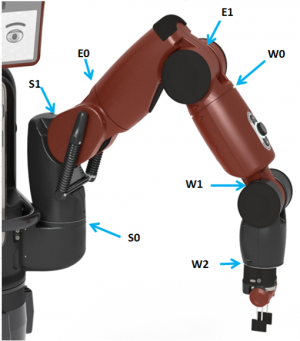
\includegraphics[width=2.5in]{imagenes/desarrollo/baxter_joint_names.png}
	\caption{Articulaciones del robot Baxter}
	\label{fig:desarrollo/joints}
\end{figure}

Cada brazo se puede controlar de manera independiente, pudiendo usar cada uno de ellos con un modo de control distinto. Los modos de control son los que se muestran a continuación:

\begin{enumerate}
\item Control por posición
\item Control por velocidad
\item Control por torque
\item Control por posición sin procesar (raw mode)
\end{enumerate}

Haciendo uso de la arquitectura de paso de mensajes que nos ofrece ROS, somos capaces de enviar en un tema (topic) tanto el modo de control que queremos usar como las características objetivos que queremos en el movimiento. El robot Baxter estará escuchando cada uno de los mensajes que le enviemos a los temas \verb|/robot/limb/left/joint_command| para el brazo izquierdo y \verb|/robot/limb/right/joint_command| para el brazo derecho. El tipo de mensaje que se envía es \verb|JointCommand|, que tiene como argumentos:

\begin{itemize}
\item mode (POSITION\_MODE=1, VELOCITY\_MODE=2, TORQUE\_MODE=3, RAW\_POSITION\_MODE=4)
\item command (lista de flotantes)
\item names (lista de nombre de articulaciones)
\end{itemize}

El modo de control para cada brazo es único, mientras que la posición/velocidad/torque deseado es único para cada articulación en cada brazo.

Aparte de enviar este tipo de mensajes, podemos definir la velocidad relativa máxima que alcanzará cada articulación en el modo de control por posición publicando al tema \verb|/robot/limb/<right/left>/set_speed_ratio| un valor entre 0 y 1.

El robot Baxter cuenta con una serie de limitaciones en cuanto a posiciones, velocidades y torques se refiere para cada articulación. Estas limitaciones se muestran en el cuadro \ref{tab:desarrollo/limits}.

\begin{table}[]
\centering
\caption{Límites articulaciones}
\label{tab:desarrollo/limits}
\begin{tabular}{cccccc}
Art.                    & (rad) Mín & (rad) Máx & (rad) Rango & (rad/s) Vel máx & (Nm/rad) \\ \hline
\multicolumn{1}{c|}{S0} & -1.7016   & +1.7016   & 3.4033      & 2.0             & 843      \\
\multicolumn{1}{c|}{S1} & -2.147    & +1.047    & 3.194       & 2.0             & 843      \\
\multicolumn{1}{c|}{E0} & -3.0541   & +3.0541   & 6.1083      & 2.0             & 843      \\
\multicolumn{1}{c|}{E1} & -0.05     & +2.618    & 2.67        & 2.0             & 843      \\
\multicolumn{1}{c|}{W0} & -3.059    & +3.059    & 6.117       & 4.0             & 250      \\
\multicolumn{1}{c|}{W1} & -1.5707   & +2.094    & 3.6647      & 4.0             & 250      \\
\multicolumn{1}{c|}{W2} & -3.059    & +3.059    & 6.117       & 4.0             & 250     
\end{tabular}
\end{table}
% Ratio de velocidad

\subsection{Control por posición}
El control por posición consiste en alcanzar las posiciones objetivo para cada una de las articulaciones. El modo de control en el mensaje JointCommand es el 1.

La orden donde todas las articulaciones se ponen en la posición 0 corresponde con el brazo totalmente estirado y con el hombro, codo y muñeca mirando hacia abajo. Las traslaciones y rotaciones se corresponden con los de la figura \ref{fig:desarrollo/joint_map}.

\begin{figure}[]
	\centering
	\begin{subfigure}[b]{0.4\textwidth}
		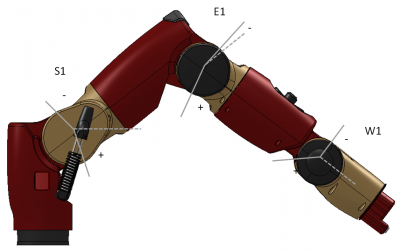
\includegraphics[width=\textwidth]{imagenes/desarrollo/baxter_range_motion1.png}
		\caption{Límites traslación}
		\label{fig:desarrollo/limits1}
	\end{subfigure}
	\begin{subfigure}[b]{0.4\textwidth}
		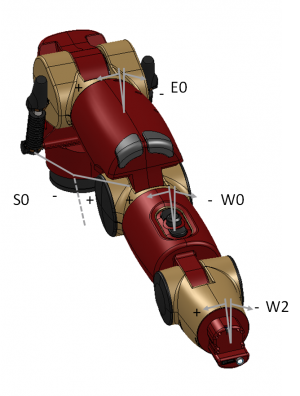
\includegraphics[width=\textwidth]{imagenes/desarrollo/baxter_range_motion2.png}
		\caption{Límites rotación}
		\label{fig:desarrollo/limits2}
	\end{subfigure}
	\caption{Límites articulaciones}
	\label{fig:desarrollo/limits}
\end{figure}

Dada la naturaleza del robot Baxter, en este modo de operación se aplican unos filtros antes de aplicar la orden de posición, a fin de evitar accidentes y otorgar una experiencia de movimiento más fluida y segura. Los filtro son los que se muestran en la figura \ref{fig:desarrollo/position_filters}.

\begin{figure}[]
	\centering
	\begin{subfigure}[b]{0.24\textwidth}
		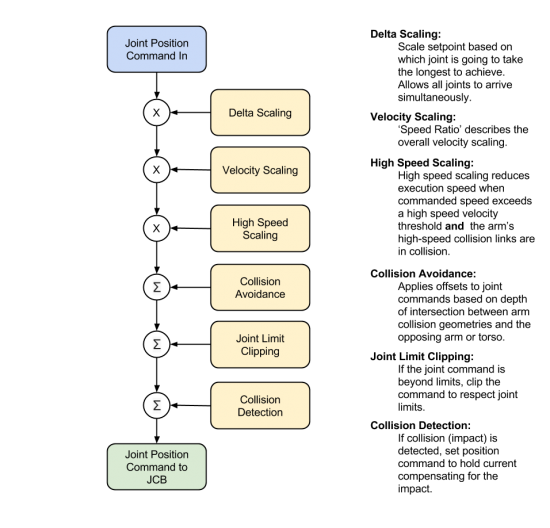
\includegraphics[trim=0 0 235 0, clip, width=\textwidth]{imagenes/desarrollo/baxter_position_filters.png}
		\caption{Control por posición}
		\label{fig:desarrollo/position_filters}
	\end{subfigure}
	\begin{subfigure}[b]{0.24\textwidth}
		\centering
		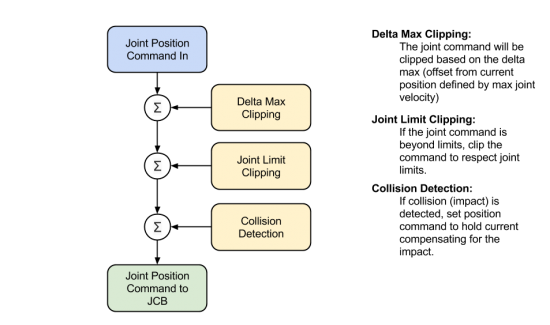
\includegraphics[trim=0 0 230 0, clip, width=\textwidth]{imagenes/desarrollo/baxter_position_raw_filters.png}
		\caption{Control por posición sin procesar}
		\label{fig:desarrollo/raw_filters}
	\end{subfigure}
	\begin{subfigure}[b]{0.24\textwidth}
		\centering
		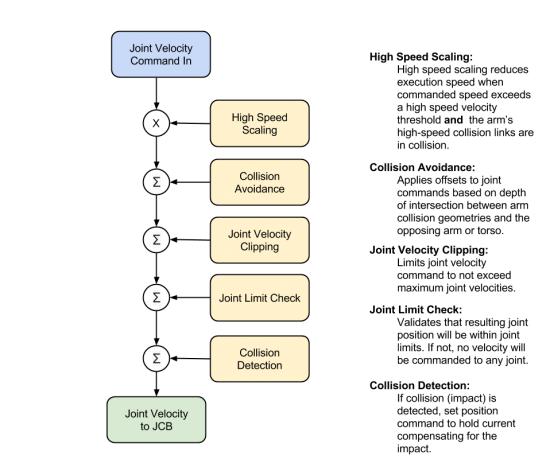
\includegraphics[trim=0 0 235 0, clip, width=\textwidth]{imagenes/desarrollo/baxter_velocity_filters.png}
		\caption{Control por velocidad}
		\label{fig:desarrollo/vel_filters}
	\end{subfigure}
	\begin{subfigure}[b]{0.24\textwidth}
		\centering
		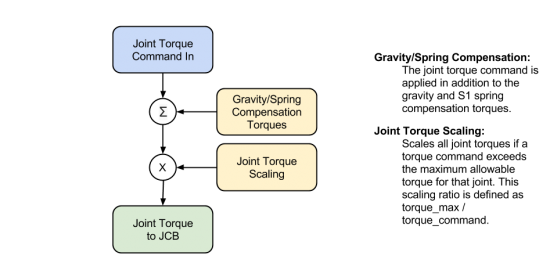
\includegraphics[trim=0 0 230 0, clip, width=\textwidth]{imagenes/desarrollo/baxter_torque_filters.png}
		\caption{Control por torque}
		\label{fig:desarrollo/torque_filters}
	\end{subfigure}
	\caption{Filtros aplicados}
\end{figure}

\begin{enumerate}
\item [Escalado delta] Consiste en escalar las posiciones objetivo en el recorrido para conseguir que todas las articulaciones lleguen al punto deseado a la vez.
\item [Escalado de velocidad] Se escala la velocidad de cada articulación en función del 'ratio de velocidad'.
\item [Escalado de alta velocidad] Para evitar colisiones entre los dos brazos moviéndose el uno en la dirección del otro, se escala la velocidad y recalcula la posición cuando ésta supera un umbral.
\item [Prevención de colisiones] Gracias a un modelo interno del robot, se limitan las posiciones de las articulaciones tales que provocarían un choque con el propio robot.
\item [Recorte de posiciones] Si las posiciones superan los límites de la articulación, estas se recortan al límite permitido.
\item [Detección de colisión] Si se detecta una colisión (con un objeto externo al robot), mantiene la última posición antes de la colisión.
\end{enumerate}

Como se puede observar, Baxter aplica unos filtros para evitar y detectar colisiones. Esta tarea se realiza de tres maneras:

\begin{itemize}
\item [Prevención] El robot ejecuta una simulación interna, donde las articulaciones y el cuerpo cuentan con unas regiones de seguridad que, al tocarse, limitan el movimiento del robot.
\item [Detección de colisión] Esto se realiza de dos maneras
\begin{enumerate}
\item [Impacto] Cuando el torque de cualquier articulación cambia bruscamente, se considera que ha habido una colisión.
\item [Retención] Cuando el torque aplicado aumenta pero la articulación no se mueve, se considera que está colisionando con un objeto inmóvil.
\end{enumerate} 
\item [Escalado de alta velocidad] Cuando la velocidad del brazo supera los 0.2 m/s, las regiones de seguridad que el robot simula internamente aumentan. Cuando se tocan estas regiones, la velocidad se escala y la posición se recalcula.
\end{itemize}

\subsection{Control por posición sin procesar}
Este modo de control, al igual que el anterior, tiene como objetivo alcanzar la posición deseada para cada articulación. Se diferencia en los filtros que aplica (figura \ref{fig:desarrollo/raw_filters}).

\begin{enumerate}
\item [Recorte de delta máximo] Recorta la posición siguiente (en el intervalo de actuación de cada articulación) a la máxima posición alcanzable a la velocidad máxima dada por la 'ratio de velocidad'.
\item [Recorte de posiciones] Al igual que en el modo de control anterior, si las posiciones superan los límites de la articulación, estas se recortan al límite permitido.
\item [Detección de colisión] Cumple la misma función que en el modo de control por posición.
\end{enumerate}

Como se puede observar, este es un modo de control más avanzado, ya que no tiene en cuenta las colisiones consigo mismo, y ofrece un movimiento más brusco al no llegar todas las articulaciones al punto destino a la vez.

El modo de control en el mensaje JointCommand es el 4.

\subsection{Control por velocidad}
En este modo de control, lo que se busca es adquirir la velocidad objetivo para cada articulación. El modo de control en el mensaje JointCommand es el 2. Al igual que en los modos anteriores, se aplican una serie de filtros (figura \ref{fig:desarrollo/vel_filters}).

\begin{enumerate}
\item [Escalado de alta velocidad] Como en el control por posición.
\item [Prevención de colisiones] Como en el control por posición.
\item [Recorte de velocidades] Se limitan las velocidades para cada articulación para que no excedan el máximo permitido.
\item [Comprobación de límites] Se comprueban los límites de las articulaciones. Si se exceden, se detiene el movimiento.
\item [Detección de colisión] Igual que en el control por posición.
\end{enumerate}

El dejar de enviar velocidades si se exceden los límites de las articulaciones es una medida de seguridad que exige al programador tener el control sobre las posiciones que puede alcanzar el brazo.

\subsection{Control por torque}
El control por torque consiste en el modo de más bajo nivel que se puede controlar el robot Baxter. Los torques que enviemos serán aplicados por los controladores, haciendo uso solamente de los siguientes filtros (figura \ref{fig:desarrollo/torque_filters}):

\begin{enumerate}
\item [Compensación] Los torques se suman a los necesarios para mantener la gravedad 0 y el muelle ubicado en la articulación s1 (traslación del hombro).
\item [Escalado de torque] Si un torque excede el torque máximo para esa articulación, escala los torques de todas las articulaciones por el factor de exceso de esa articulación (torque\_max/torque).
\end{enumerate}

La compensación de la gravedad se puede desactivar mandando un mensaje vacío al tema \verb|/robot/limb/right/suppress_gravity_compensation| para el brazo derecho, o \verb|/robot/limb/left/suppress_gravity_compensation| para el brazo izquierdo.

De esta manera, un torque aplicado de 0 en todas las articulaciones, mantendrá el brazo en un estado de gravedad 0 si la compensación esta activa. De no estarlo, el brazo caerá en peso muerto.
	

\section{Obtención de datos}
A fin de conseguir un controlador basado en el propio de Baxter, se ha de obtener una base de datos de movimientos de los cuales aprender. Esta base de datos consistirá en las posiciones, velocidades y torques registradas por el robot, así como de las órdenes enviadas sobre la posición deseada y la ratio de velocidad deseada.

Para ello, haremos uso de la interfaz de programación de aplicaciones (API) para el lenguaje Python que ofrece Baxter. Esta API cuenta con una serie de funciones que nos permitirán mover el robot abstrayéndonos de las instrucciones ROS que ejecuta. Para la toma de datos, se hará uso de la herramienta \verb|rosbag| que proporciona ROS.

\subsection{API de Python}
La API tiene como objetivo disponer una interfaz basada en el lenguaje de programación Python para controlar y monitorizar el robot Baxter, ejecutando en su base las correspondientes instrucciones ROS. Para ello, cuenta con una serie de módulos orientados a los distintos componentes del robot (brazos, pinzas, cámara...).

Se hará uso del módulo \verb|brazo| para realizar el movimiento del mismo. Por motivos de disposición del robot en el laboratorio, se extraerá la base de datos haciendo uso del brazo izquierdo.

Dentro de este módulo, se hará uso de las funciones \verb|set_joint_position_speed(speed)| y \verb|move_to_joint_positions(positions)|. La primera controlará la velocidad máxima relativa para cada articulación, mientras que la segunda moverá el brazo a la posición deseada. Esta función cuenta además con un intervalo de tiempo máximo para realizar el movimiento. Que el tiempo máximo se agote será indicador de que el robot no puede alcanzar la posición deseada (está colisionando consigo mismo).

Un dato a tener en cuenta es que la función \verb|move_to_joint_positions(positions)| realiza un filtro paso baja de la diferencia de posiciones (actual y deseada) en el tiempo, ofreciendo un movimiento más fluido.

\subsection{rosbag}
\verb|rosbag| es una herramienta para grabar el paso de mensajes realizados sobre los temas que se le ofrecen como parámetros. Tiene la peculiaridad de grabar los mensajes enteros, lo que significa que registra tanto el mensaje en sí, como la marca temporal y de secuencia que cada mensaje tiene asociadas. Esto será útil más adelante para sincronizar los mensajes de posición y velocidad relativa deseadas (generadas en el ordenador local) con los mensajes de posición, velocidad y torque generados por el robot y enviados por tcp/ip al ordenador.

Los temas que registraremos serán:

\begin{itemize}
\item \verb|/robot/joint_states| Tanto la posición como la velocidad y torque de las articulaciones del brazo izquierdo.
\item \verb|/robot/limb/left/set_speed_ratio| Ratio de velocidad deseada.
\item \verb|/robot/limb/left/joint_command| Posiciones deseadas.
\end{itemize}

\subsection{Ejecución}
El espacio vectorial de las siete dimensiones formadas por cada una de las articulaciones del Baxter se muestreará de manera uniforme, a fin de obtener una base de datos representativa del controlador que estamos aprendiendo. Esto significa que, para cada movimiento, se elegirán siete posiciones objetivo (una por articulación) de acuerdo a una distribución uniforme sobre el rango de cada articulación. De igual manera se elegirá una ratio de velocidad objetivo con distribución uniforme entre 0 y 1. El tiempo máximo empleado para cada movimiento será de 15 segundos, ya que es tiempo suficiente para permitir el movimiento entre puntos distantes entre sí a una velocidad baja.

Para realizar una primera aproximación de la manera en la que la red neuronal aprende, se han realizado una serie de base de datos con distintas características, para así aislar los potenciales problemas con los que nos enfrentamos.

\begin{itemize}
\item [Una articulación] Se ha aislado el problema del tamaño del espacio a muestrear reduciéndolo a una de las siete articulaciones. El resto de las articulaciones se mantienen quietas en la posición cero.
\item [5 segundos] En lugar de limitar el tiempo para cada movimiento a 15 segundos, se limita a 5 segundos, para así aislar el problema de desdoblar la red en un intervalo de tiempo tan alto.
\item [0.5 seg. ratio vel. 1] Es el caso más simple para entrenar la red. Se mueve una sola articulación (el resto se ubican en la posición 0) a máxima velocidad (relación de velocidad 1) durante 0.5 segundos. De esta manera obtenemos una base de datos muy amplia (más de 120 posiciones objetivo por minuto) con el problema del tamaño del espacio y del desdoblamiento temporal muy limitados.
\end{itemize}

Adicionalmente, se ha obtenido un conjunto de datos con combinaciones de distintas articulaciones, así como del brazo con las pinzas anexas.

\subsection{Tratamiento}
Una vez obtenida las distintas bases de datos, se preparan para la fase de entrenamiento y evaluación de la red neuronal.

\subsubsection{Ficheros .bag}
El primer paso consiste en transformar la base de datos en tipos de datos que entienda el lenguaje de programación Python.

Los ficheros obtenidos con \verb|rosbag| tienen la extensión \verb|.bag|, y consisten en ficheros conteniendo mensajes sobre los que se iteran. De esta manera, iteramos sobre cada mensaje y leemos su contenido, que consiste en el tema del cual proviene el mensaje, una marca temporal de su recepción por \verb|rosbag|, y del mensaje en sí mismo.

La marca temporal corresponde al tiempo del reloj interno del ordenador en el cual se recibe el mensaje. Dado que la conexión entre el robot y el ordenador se realiza por tcp/ip, este tiempo diferirá del de generación en el robot. Para paliar con este problema, \verb|ROS| dispone una marca temporal dentro del cuerpo del mensaje con el instante de creación del mensaje en el robot (de acuerdo a su reloj interno), además de un número de secuencia para ordenar los mensajes en el ordenador.

\paragraph{Error en frecuencia}
Gracias a esta información, se percibió un error en frecuencia entre el reloj del ordenador y el del robot. Esto significa que, a una frecuencia de generación de mensajes de 100 Hz, el ordenador generó 100 posiciones y velocidades deseadas por segundo (suponiendo que es el que tiene el reloj ajustado correctamente), mientras que el robot generó 99 posiciones, velocidades y torques actuales. Para solventar este problema, en primera instancia se representó gráficamente la diferencia de mensajes obtenidos por parte del ordenador y el robot en función del tiempo (figura \ref{fig:desarrollo/diferencia}).

\begin{figure}[]
	\centering
	\begin{subfigure}[b]{0.45\textwidth}
		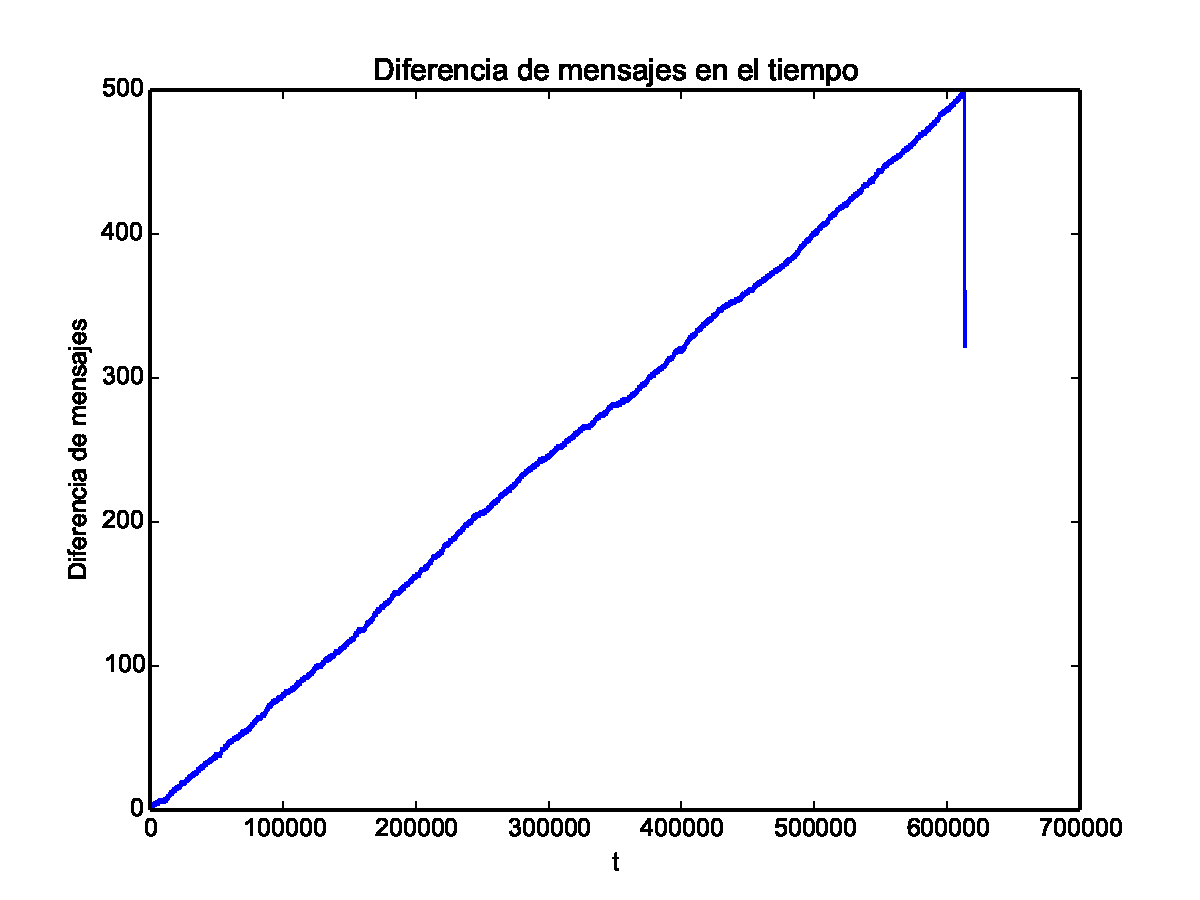
\includegraphics[width=\linewidth]{imagenes/desarrollo/diferencia.pdf}
		\caption{Señal sin procesar}
		\label{fig:desarrollo/diferencia}
	\end{subfigure}
	\begin{subfigure}[b]{0.45\textwidth}
		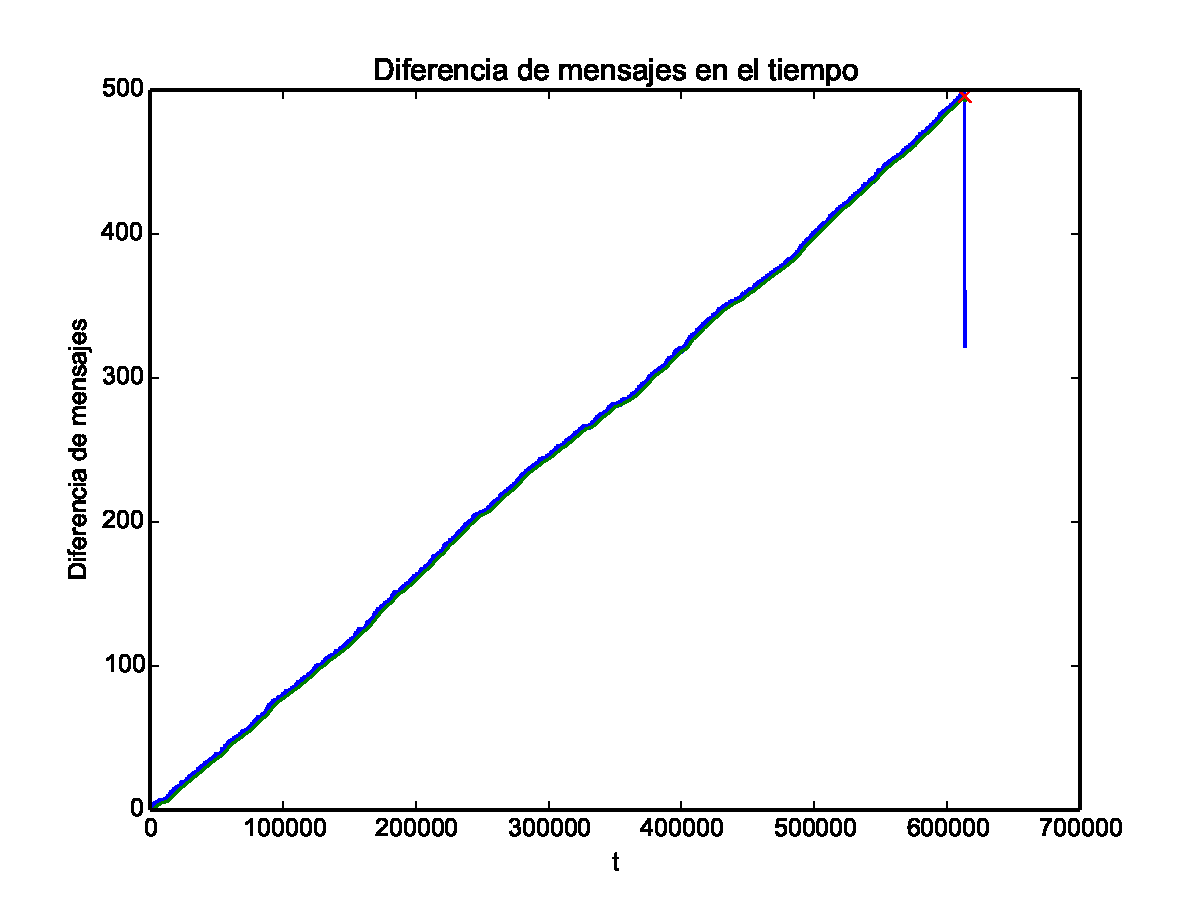
\includegraphics[width=\linewidth]{imagenes/desarrollo/diferenciafilt.pdf}
		\caption{Señal filtrada paso baja}
		\label{fig:desarrollo/diferenciafilt}
	\end{subfigure}
	\caption{Diferencia de mensajes recibidos del ordenador y del robot}
\end{figure}

Como se puede observar, esta diferencia crece con el tiempo, lo que significa que el ordenador genera mensajes a mayor velocidad que el robot. Es cuando el ordenador deja de generar mensajes cuando esta diferencia cae en picado, momento en el cual, los mensajes generados por el robot dejarán de corresponderse con las posiciones deseadas y pasarán a corresponderse con las posiciones, velocidades y torques del robot manteniendo la última posición alcanzada.

Por lo tanto, el objetivo será encontrar el momento en el que ocurre dicha bajada, es decir, el pico. El problema surge cuando la señal no es monótona, sino que, como se observa en la figura \ref{fig:desarrollo/diferenciadetalle}, crece y decrece en intervalos temporales pequeños (debido a la naturaleza a ráfagas de la señal). Para paliar con este inconveniente, se realiza un filtrado paso baja (con un filtro de media móvil) que elimine dicha componente frecuencial. El resultado es el que se observa en las figuras \ref{fig:desarrollo/diferenciafilt} y \ref{fig:desarrollo/diferenciadetallefilt}. A partir de esta señal, solo queda seleccionar el valor máximo de la misma. El valor obtenido es el número de mensaje recibido hasta el cual los mensajes son válidos.

\begin{figure}[]
	\centering
	\begin{subfigure}[b]{0.45\textwidth}
		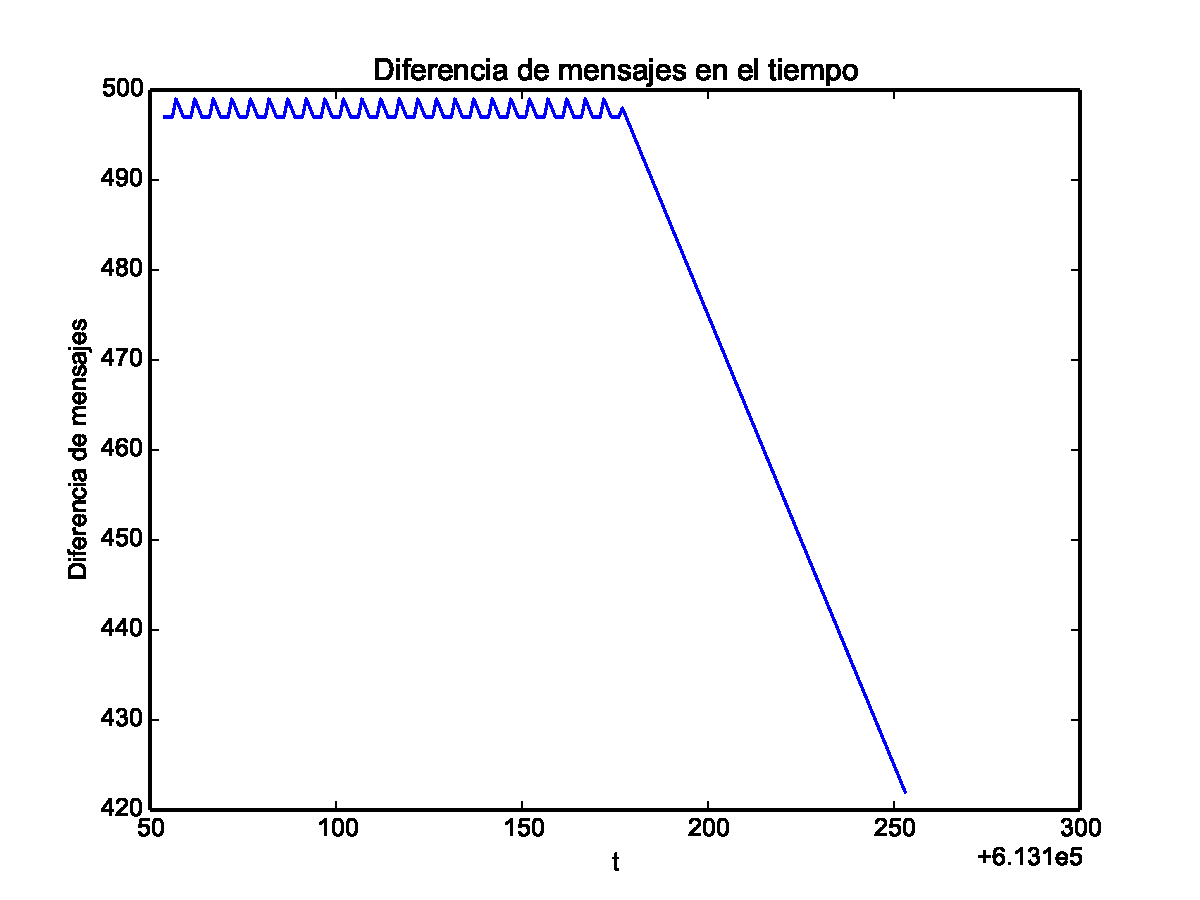
\includegraphics[width=\linewidth]{imagenes/desarrollo/diferenciadetalle.pdf}
		\caption{Señal sin procesar}
		\label{fig:desarrollo/diferenciadetalle}
	\end{subfigure}
	\begin{subfigure}[b]{0.45\textwidth}
		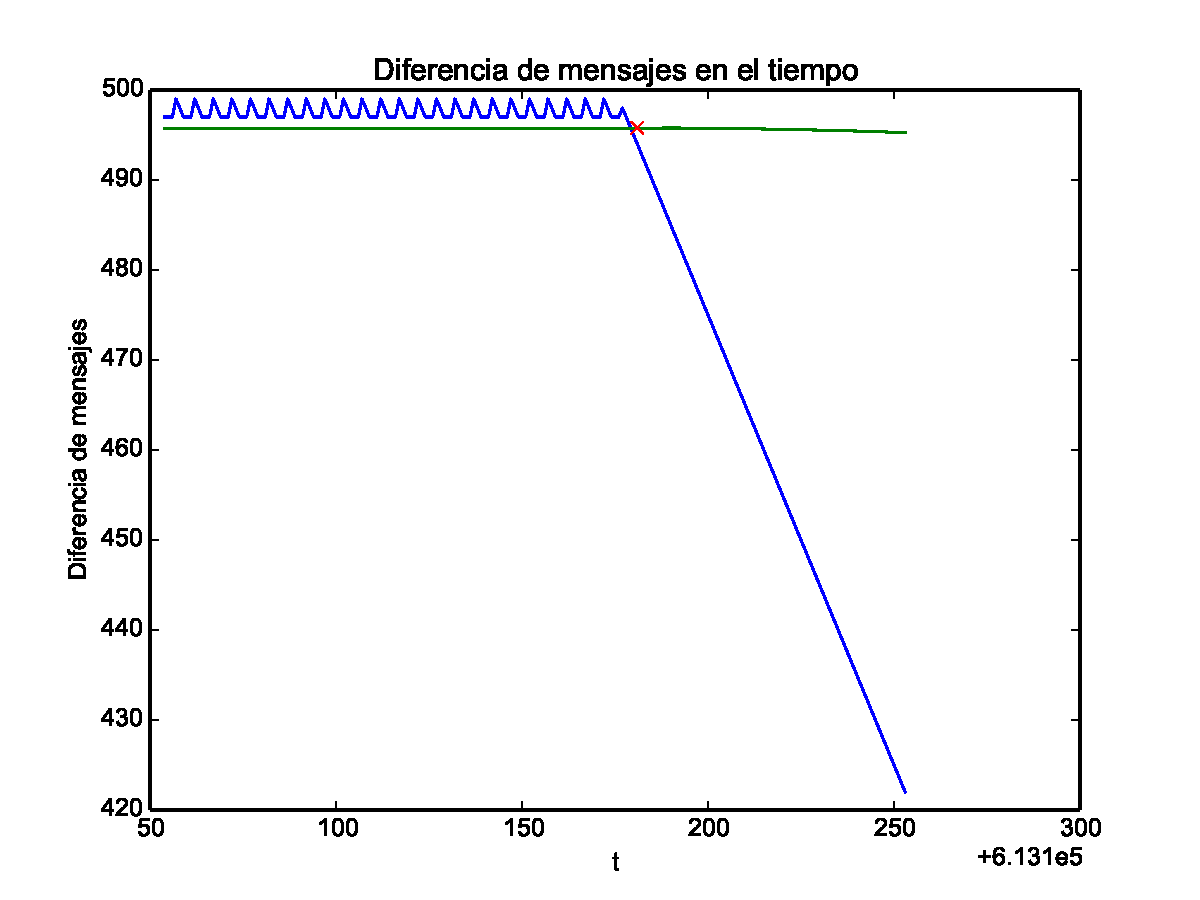
\includegraphics[width=\linewidth]{imagenes/desarrollo/diferenciafiltdetalle.pdf}
		\caption{Señal filtrada paso baja}
		\label{fig:desarrollo/diferenciadetallefilt}
	\end{subfigure}
	\caption{Detalle de diferencia de mensajes recibidos del ordenador y del robot}
\end{figure}

Dado que el control lo vamos a realizar desde el ordenador, adaptamos los mensajes recibidos al mismo. Esto lo hacemos mediante interpolación lineal en las posiciones, velocidades y torques recibidos.

De esta manera, se obtienen vectores de la misma longitud (en el tiempo) tanto enviados como recibidos.

\paragraph{Ráfagas}
También se percibió la llegada a ráfagas en los mensajes provenientes del robot. Esto no supone un problema para preparar los datos, pero sí lo es a la hora de realizar un controlador realimentado que requiere la información que proporciona el robot sin desfases. El controlador propuesto en este trabajo no es realimentado, pero de serlo, una posible solución sería implementar el controlador en el propio robot (no ejecutarlo en el ordenador), aunque para ello habría que tomar nuevamente la base de datos o ajustarla a la frecuencia de generación de mensajes del robot. Otra posible solución consistiría en un predictor de posiciones y velocidades que ofrezcan al controlador esta información cuando no disponga de la misma. Por ejemplo, supongamos que en un instante concreto, llega una ráfaga de tres posiciones, velocidades y torques provenientes del robot. Esto significa que, dos instantes anteriores, el ordenador no ha obtenido ninguna información, por lo que la última posición, velocidad y torques conocidos son los obtenidos hace dos instantes temporales. En este caso, el predictor generaría 2 posiciones y velocidades (los torques serían la salida del sistema) para los instantes temporales que no disponen de información directa.


\section{Red Neuronal}
A continuación se estudia la viabilidad de la implementación de un controlador a partir del propio de Baxter basado en redes neuronales profundas (deep learning).
\subsection{Viabilidad}
El primer problema a enfrentarse es el de demostrar que la red neuronal es capaz de aprender algo de los datos extraídos del controlador del Baxter. Por la capacidad de detectar colisiones sabemos que es un sistema realimentado, posiblemente con un controlador PID.

Se podría realizar un controlador donde el modelo dinámico (controlador feedforward) fuera desempeñado por la red neuronal, y donde la realimentación fuera desempeñada por el controlador PID. También podría implementarse la realimentación como otra red neuronal, pero ambas aproximaciones tienen el problema de enfrentarse a la realimentación y al tiempo real (a una frecuencia de realimentación de 100Hz). Las redes neuronales profundas tienen el problema de ser pesadas en el cómputo (debido a las no linealidades usadas para la activación de las neuronas), poniendo en riesgo la capacidad de afrontar el problema en tiempo real.

Es por esto por lo que se decide hacer un controlador sin realimentación, donde los datos de entrada sean posiciones objetivo, posiciones en el momento de iniciar el movimiento, y velocidad objetivo, siendo los de salida una sucesión de torques a aplicar para alcanzar la posición deseada.

Para ello se elige una arquitectura basada en redes neuronales realimentadas, ya que las no realimentadas tienen la limitación de generar la misma salida ante la misma entrada, y siendo nuestra entrada única (debido a que el sistema no es realimentado), generaríamos siempre la misma salida, en vez de la sucesión de torques deseada.

Nos encontramos con el problema de, si el controlador implementado por Baxter es realimentado, ¿puede un modelo no realimentado aprender de este? % Quitar pregunta?
El controlador del Baxter tiene una estructura como la mostrada en la figura \ref{fig:desarrollo/feedforward_controller}. El funcionamiento es el siguiente:

\begin{enumerate}
\item El controlador realimentado genera una señal torque a partir de la realimentación de posición del sistema y la posición deseada.
\item El controlador feedforward tiene en cuenta el modelo interno del robot y ajusta la señal de control generada por el controlador realimentado.
\item Se transmite la señal y el robot genera el torque enviado.
\item La aplicación genera una nueva posición que es recibido por los sensores y usado para la realimentación.
\end{enumerate}

\tikzstyle{block} = [draw, fill=blue!20, rectangle, 
    minimum height=3em, minimum width=6em]
\tikzstyle{sum} = [draw, fill=blue!20, circle, node distance=1cm]
\tikzstyle{input} = [coordinate]
\tikzstyle{output} = [coordinate]
\tikzstyle{pinstyle} = [pin edge={to-,thin,black}]
\begin{figure}[]
	\centering
	\deactivatequoting
	\begin{tikzpicture}[auto, node distance=2cm,>=latex']
	    % We start by placing the blocks
	    \node [input, name=input] {};
	    \node [sum, right of=input] (sum) {};
	    \node [block, right of=sum] (controller) {Controller};
	    \node [sum, right of=controller] (sum2) {};
	    \node [block, right of=sum2, pin={[pinstyle]above:Disturbances},
	          node distance=3cm] (system) {System};
	    % We draw an edge between the controller and system block to 
	    % calculate the coordinate u. We need it to place the measurement block. 
	    \draw [->] (sum2) -- node[name=u] {$u$} (system);
	    \node [output, right of=system] (output) {};
	    \node [block, below of=u] (measurements) {Measurements};
	
	    % Once the nodes are placed, connecting them is easy. 
	    \draw [draw,->] (input) -- node {$r$} (sum);
	    \draw [->] (sum) -- node {$e$} (controller);
 	    \draw [->] (controller) -- node {$e$} (sum2);
	    \draw [->] (system) -- node [name=y] {$y$}(output);
	    \draw [->] (y) |- (measurements);
	    \draw [->] (measurements) -| node[pos=0.99] {$-$} 
	        node [near end] {$y_m$} (sum);
	\end{tikzpicture}
	\caption{Sistema de control de Baxter}
	\label{fig:desarrollo/feedforward_controller}
	\activatequoting
\end{figure}

El controlador realimentado no es más que un sistema (lineal o no) que a ciertas entradas genera ciertas salidas (en función de su historia o no). El controlador feedforward igualmente es un sistema que tiene en cuenta el modelo dinámico del robot, y por lo tanto los dos sistemas son reproducibles por una red neuronal. Por último, tenemos la realimentación, y es en este aspecto, donde la red neuronal tendrá que aprender a producir estimaciones de la salida provocada (posiciones de las articulaciones) al aplicar los torques.

Por lo tanto, la viabilidad de nuestro controlador depende de la capacidad de la red para generar dicha estimación de la realimentación.

Es por ello por lo que se utilizarán redes neuronales recurrentes, ya que tanto el controlador realimentado, como el feedforward, como la realimentación en sí misma son sistemas que dependen de la historia de las señales de las que dependen, y esto es exactamente lo que hacen este tipo de redes.

% explicar pid
% explicar controlador feedforward
% explicar error distal
% contar historia del proyecto:
% 	- obtener parámetros óptimos del PID

% ros: mensajes con marcas temporales y secuencias
% rosbag

% disposición del robot, conectado directamente al ordenador (y no a un router)
% Referenciar imágenes pertenecientes a la página de baxter
% ¿Números con números, o con letras?
% Cómo escribir Hz correctamente (estilo latex)
% Cómo referirme al ordenador con el que controlo el Baxter (lo estoy llamando ordenador)
% Cómo referirme al Baxter (lo llamo Baxter, robot, robot Baxter)
% Utilizar la voz pasiva (se hizo, se ejecutó...), o la primera persona del plural (hicimos, ejecutamos...)?